\documentclass[review]{elsarticle}

\usepackage{lineno,hyperref}
\modulolinenumbers[5]

\journal{Journal of \LaTeX\ Templates}

%%%%%%%%%%%%%%%%%%%%%%%
%% Elsevier bibliography styles
%%%%%%%%%%%%%%%%%%%%%%%
%% To change the style, put a % in front of the second line of the current style and
%% remove the % from the second line of the style you would like to use.
%%%%%%%%%%%%%%%%%%%%%%%

%% Numbered
%\bibliographystyle{model1-num-names}

%% Numbered without titles
%\bibliographystyle{model1a-num-names}

%% Harvard
%\bibliographystyle{model2-names.bst}\biboptions{authoryear}

%% Vancouver numbered
%\usepackage{numcompress}\bibliographystyle{model3-num-names}

%% Vancouver name/year
%\usepackage{numcompress}\bibliographystyle{model4-names}\biboptions{authoryear}

%% APA style
%\bibliographystyle{model5-names}\biboptions{authoryear}

%% AMA style
%\usepackage{numcompress}\bibliographystyle{model6-num-names}

%% `Elsevier LaTeX' style
\bibliographystyle{elsarticle-num}
%%%%%%%%%%%%%%%%%%%%%%%

\begin{document}

\begin{frontmatter}

\title{Elsevier \LaTeX\ template\tnoteref{mytitlenote}}
\tnotetext[mytitlenote]{Fully documented templates are available in the elsarticle package on \href{http://www.ctan.org/tex-archive/macros/latex/contrib/elsarticle}{CTAN}.}

%% Group authors per affiliation:
\author{Elsevier\fnref{myfootnote}}
\address{Radarweg 29, Amsterdam}
\fntext[myfootnote]{Since 1880.}

%% or include affiliations in footnotes:
\author[mymainaddress,mysecondaryaddress]{Elsevier Inc}
\ead[url]{www.elsevier.com}

\author[mysecondaryaddress]{Global Customer Service\corref{mycorrespondingauthor}}
\cortext[mycorrespondingauthor]{Corresponding author}
\ead{support@elsevier.com}

\address[mymainaddress]{1600 John F Kennedy Boulevard, Philadelphia}
\address[mysecondaryaddress]{360 Park Avenue South, New York}

\begin{abstract}
This template helps you to create a properly formatted \LaTeX\ manuscript.
\end{abstract}

\begin{keyword}
\texttt{elsarticle.cls}\sep \LaTeX\sep Elsevier \sep template
\MSC[2010] 00-01\sep  99-00
\end{keyword}

\end{frontmatter}

\linenumbers
%%%%%%%%%%%%%%%%%%%%%%%%%%%%%%%%%%%%%%%%%%%%%%%%%%%%%%%%%
%%%%%%%%%%%%%%%%%%%%%%%%%%%%%%%%%%%%%%%%%%%%%%%%%%%%%%%%%



%%%%%%%%%%%%%%%%%%%%%%%%%%%%%%%%%%%%%%%%%%%%%%%%%%%%%%%%%
\section{Introduction} 
\texttt{State the objectives of the work and provide an adequate background, avoiding a detailed literature survey or a summary of the results.}
The constantly growing amounts of data and an emerging trend of incorporating unstructured  data into analytics is bringing new challenges to Business Intelligence (BI). Traditional Business Intelligence (BI) solutions fall short in different aspects. Firstly, they focus only on structured data and disregard the increasing amount of information hidden in unstructured data. Secondly, they focus solely on quantitative analysis of the data: qualitative aspects, like structural dependencies in the data, are neglected. 

In the EU funded research project CUBIST, which ran from October 2010 to September 2013, those two drawbacks have ben addressed. CUBIST?s approach was to complement traditional BI solutions. The CUBIST project developed methodologies and a platform that combines essential features of Semantic Technologies and BI. The most-prominent deviations from traditional BI-platforms are:
\begin{itemize}
\item The data persistency layer in the CUBIST-prototype based on a BI enabled triple store, thus CUBIST enables a user to perform BI operations over semantic data.
\item  In addition to some traditional charts, CUBIST provides novel graph-based visualizations to analyse the data.  As mathematical foundation for meaningfully clustering the data, Formal Concept Analysis is used.
\end{itemize}

From a user?s perspective, CUBIST provides three different means to access the data:
\begin{itemize}
\item Factual search: First of all, using a semantic search allows the user to specifically the query the data, in order to retrieve small or large sets of entities which satisfying user-defined constraints. 
\item Explorative search: A graph-based view allows the user to interactively explore the data.
\item Visual analytics: Clusters and aggregations of data can be visually analyzed using traditional charts or novel visualizations. The selection of the visualized data as well as the visualizations are highly interactive, thus CUBIST provides ?BI as a self-service?.
\end{itemize}

A first, general diagram which depict the differences between traditional BI and CIBUST is depicted below in Figure \ref{fig:classical_v_semantic}.

CUBIST was the joint effort of seven partners, namely the project coordinator SAP SE (SAP AG during the project runtime, SAP, Germany), Ontotext (ONTO, Bulgaria), Sheffield Hallam University (SHU, UK), Centrale Rechereche S.A. (CRSA, France), Heriot-Watt University (HWU, UK), Space Applications Services (SAS, Belgium), Innovantage (INN, UK). 

SAP, ONTO, SHU and CRSA served as technological partners. During the project, they have developed a web-based prototype with the following capabilities: 
\begin{itemize}
\item Unstructured and structured data is federated in a triple store.
\item The prototype supports different information needs, i.e. searching for data, exploring and navigating in the data, and analysing the data.
\item The prototype supports ``BI as a selfservice" via comprehensive filter mechanisms and leveraging the semantics of the data.
\item The Visual Analytics of CUBIST consists of an extensive set of novel and highly interactive diagrams which allow both the quantitative and qualitative analysis of the data.
\end{itemize}

Use cases have been provided by the use case partners HWU, SAS, and INN. They have provided requirements and data sets at the beginning and constant feedback during the project lifespan, until they have finally evaluated the prototype at the project end. In CUBIST, HWU explored the semantic representation of biomedical data from a biomedical atlas and a gene expression database. SAS investigated telemetry data of a specific research device in space they monitor in mission control rooms. Finally, INN provided a job market use case which combined information from job advertisements crawled by CUBIST and an existing firmographic database.

This paper describes the approach of CUBIST, the prototype which has been developed, and the results oft he project ?particularly the evaluation in detail. The project as such, particularly its setup, the use cases, core technologies, and key theses are provided in section XXX. The prototype is described both in terms of technology and architecture as well as in terms of capabilities is described in section XXX: The results oft he project, particularly the results of the evaluation, are described in Section XXX. 

\begin{figure}[htbp]
   \centering
   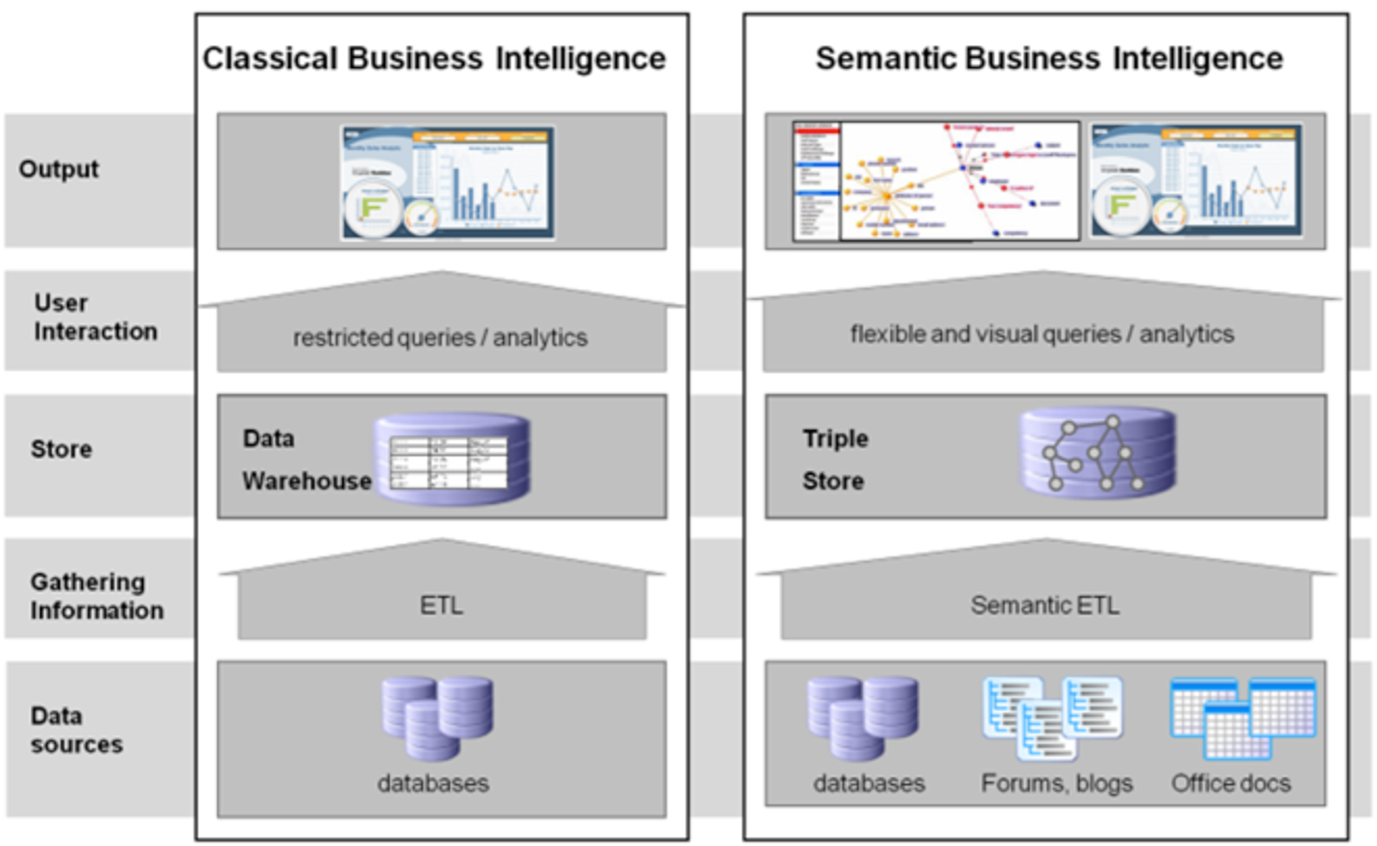
\includegraphics[width=8cm]{images/classicBI_vs_semanticBI} % requires the graphicx package
   \caption{Infographic comparing classical Business Intelligence approach against Semantic Business Intelligence.}
   \label{fig:classical_v_semantic}
\end{figure}

%%%%%%%%%%%%%%%%%%%%%%%%%%%%%%%%%%%%%%%%%%%%%%%%%%%%%%%%%
\section{Material and methods} 
\texttt{Provide sufficient detail to allow the work to be reproduced. Methods already published should be indicated by a reference: only relevant modifications should be described.}

%%%%%%%%%%%%%%%%%%%%%%%%%%%%%%%%%%%%%%%%%%%%%%%%%%%%%%%%%
\section{Theory/calculation} 
\texttt{A Theory section should extend, not repeat, the background to the article already dealt with in the Introduction and lay the foundation for further work. In contrast, a Calculation section represents a practical development from a theoretical basis.}

%%%%%%%%%%%%%%%%%%%%%%%%%%%%%%%%%%%%%%%%%%%%%%%%%%%%%%%%%
\section{Results} 
\texttt{Results should be clear and concise.}

%%%%%%%%%%%%%%%%%%%%%%%%%%%%%%%%%%%%%%%%%%%%%%%%%%%%%%%%%
\section{Discussion} 
\texttt{This should explore the significance of the results of the work, not repeat them. A combined Results and Discussion section is often appropriate. Avoid extensive citations and discussion of published literature.}

%%%%%%%%%%%%%%%%%%%%%%%%%%%%%%%%%%%%%%%%%%%%%%%%%%%%%%%%%
\section{Conclusions} 
\texttt{The main conclusions of the study may be presented in a short Conclusions section, which may stand alone or form a subsection of a Discussion or Results and Discussion section.}

%%%%%%%%%%%%%%%%%%%%%%%%%%%%%%%%%%%%%%%%%%%%%%%%%%%%%%%%%
\section{Vitae} 



%%%%%%%%%%%%%%%%%%%%%%%%%%%%%%%%%%%%%%%%%%%%%%%%%%%%%%%%%
%%%%%%%%%%%%%%%%%%%%%%%%%%%%%%%%%%%%%%%%%%%%%%%%%%%%%%%%%

\section{Bibliography styles}

There are various bibliography styles available. You can select the style of your choice in the preamble of this document. These styles are Elsevier styles based on standard styles like Harvard and Vancouver. Please use Bib\TeX\ to generate your bibliography and include DOIs whenever available.

Here are two sample references: \cite{Feynman1963118,Dirac1953888}.

\section*{References}

\bibliography{mybibfile}

\end{document}